\chapter{Simulace očních vad pohledů prototypu v nástroji Figma}
\label{appendix:simulations-of-eye-defects}
\noindent
Na světě v současné době s poruchami zraku bojuje minimálně 2,2 miliardy lidí, \cite{WorldReportOnVision} což není malá skupina a proto je důležité se zaměřit na téma, zda je výsledný produkt použitelný pro lidi, kteří mají problémy s vnímáním barev. Může se stát, že se jednotlivé barvy nebudou mít dostatečný kontrastní poměr a pro člověka s poruchou vnímání barev se tyto barvy mohou jevit jako totožné, což zapříčiní, že daná aplikace pro ně bude nepoužitelná.

\section{Simulace očních vad pro hlavní stranu}
\noindent
Achromatopsie znamená úplnou barvoslepost, kdy oko nedokáže vnímat žádné barvy, což vede k tomu, že vidění je omezeno pouze na černou a bílou s odstíny šedi.
\begin{figure}[htbp]
\centering
    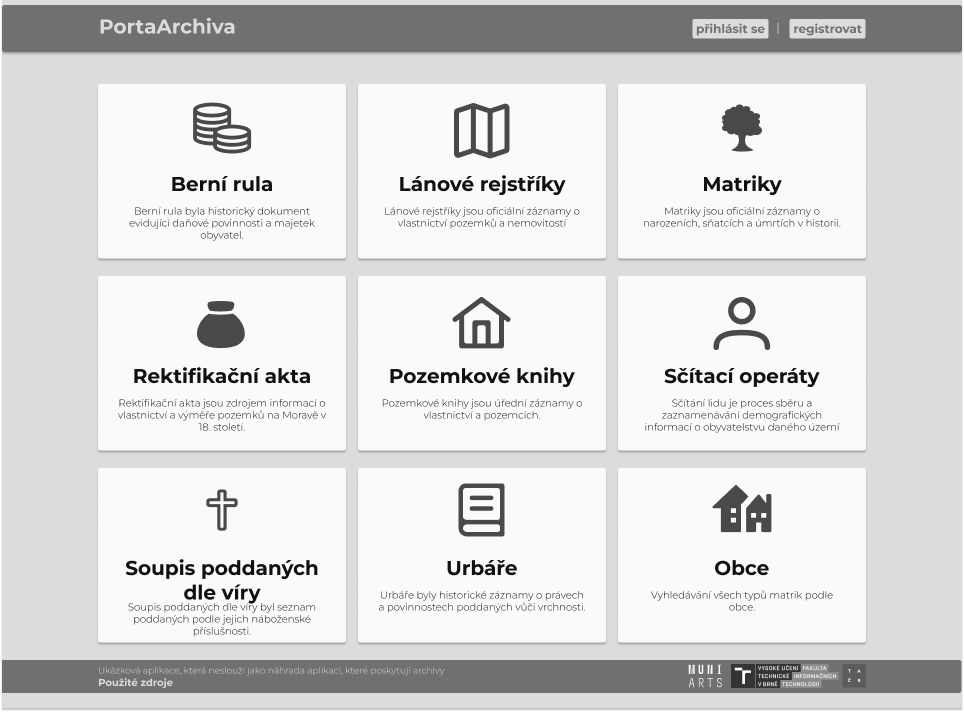
\includegraphics[scale=.35]{obrazky-figures/testing/figma-eye-defects/Main - Achromatopsia.png}
    \caption{Hlavní strana - simulace achromatopsie}
\end{figure}

\newpage
\noindent
Oční vada, při které se paprsky světla, které procházejí čočkou lidského oka, sbíhají před sítnicí. Tím není na sítnici vytvořen ostrý obraz.
\begin{figure}[htbp]
\centering
    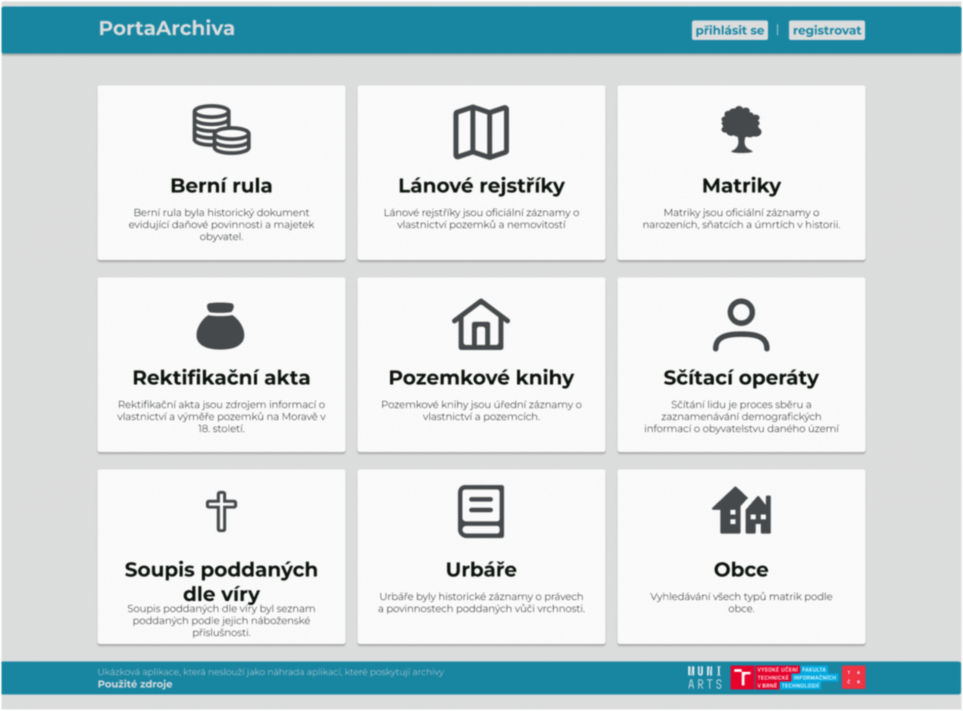
\includegraphics[scale=.35]{obrazky-figures/testing/figma-eye-defects/Main - Blurred.png}
    \caption{Hlavní strana - simulace krátkozrakosti}
\end{figure}

\noindent
Světloplachost (fotofobie) se projevuje pocitem oslnění u pacientů i při pohledu za běžných světelných podmínek.
\begin{figure}[htbp]
\centering
    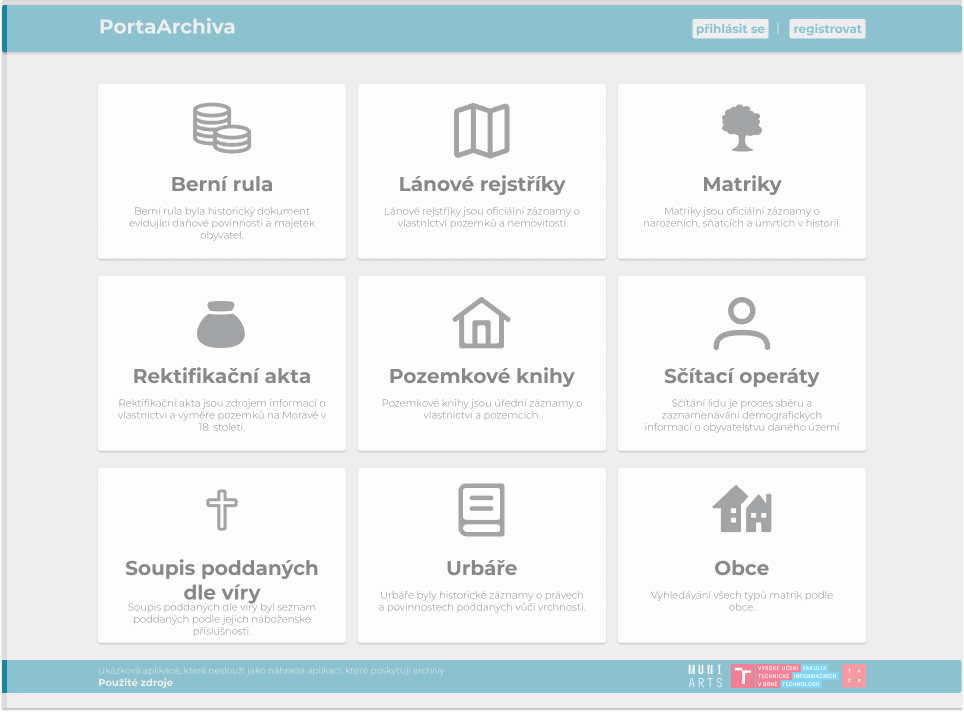
\includegraphics[scale=.35]{obrazky-figures/testing/figma-eye-defects/Main - Bright Light.png}
    \caption{Hlavní strana - simulace fotofobie}
\end{figure}

\newpage
\noindent
Deuteranopie je forma poruchy barvocitu, při níž pacient není schopen vnímat zelenou barvu.
\begin{figure}[htbp]
\centering
    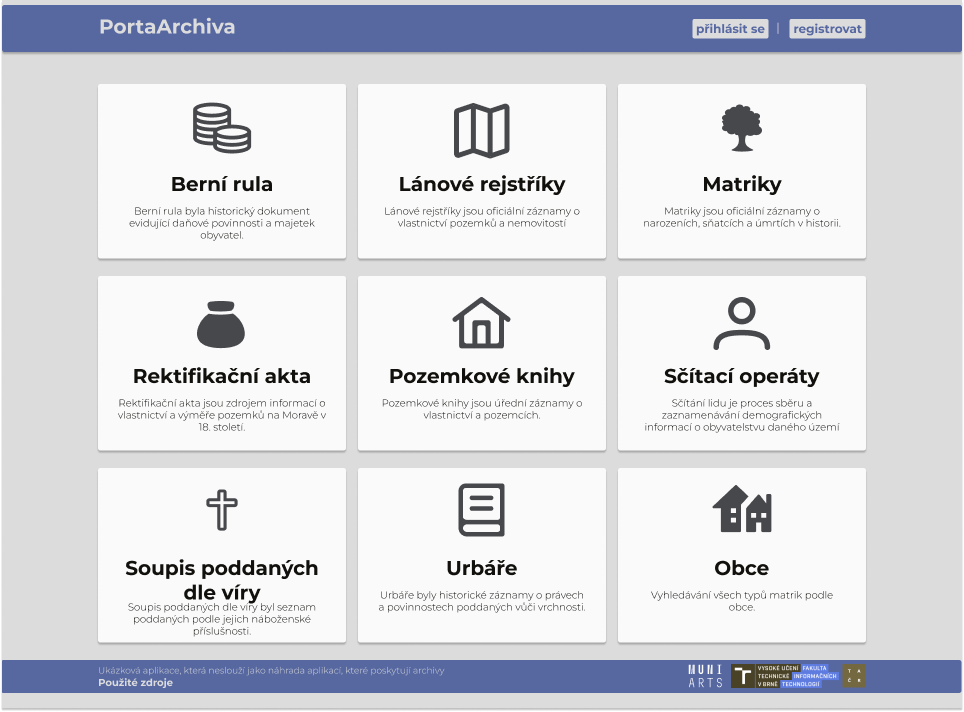
\includegraphics[scale=.35]{obrazky-figures/testing/figma-eye-defects/Main - Deuteranopia.png}
    \caption{Hlavní strana - simulace Deuteranopie}
\end{figure}

\noindent
Diplopie je porucha, při níž pacient vnímá dva obrazy jednoho předmětu současně. Toto onemocnění se může také projevovat krátkodobým rozmazaným viděním.
\begin{figure}[htbp]
\centering
    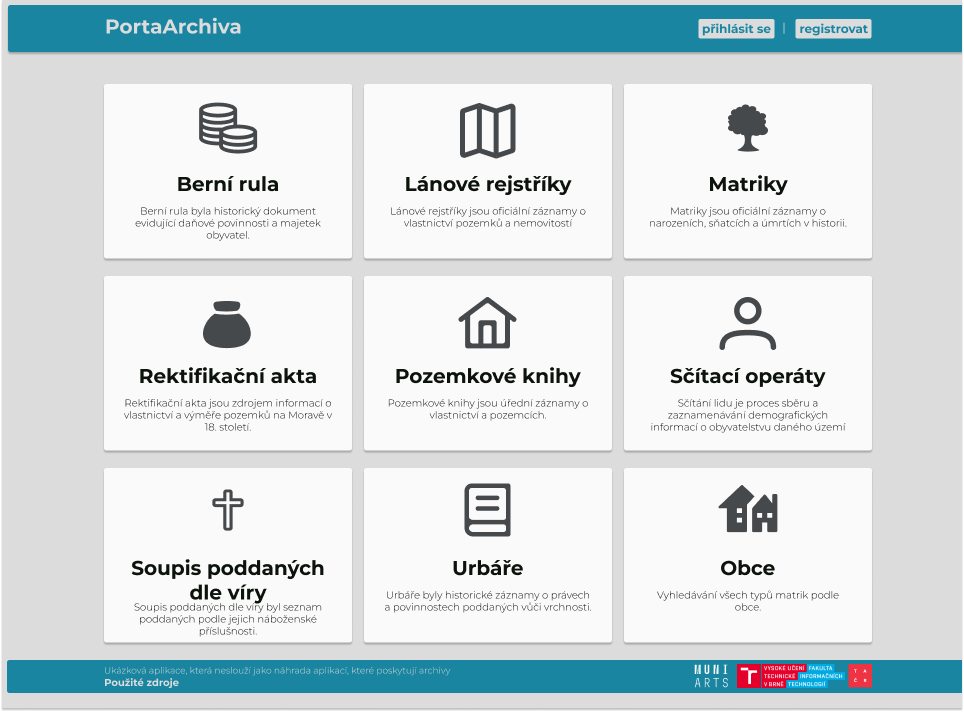
\includegraphics[scale=.35]{obrazky-figures/testing/figma-eye-defects/Main - Ghosting.png}
    \caption{Hlavní strana - simulace Diplopie}
\end{figure}

\newpage
\noindent
Zelený zákal, lékařsky označovaný jako glaukom, je onemocnění, které způsobuje trvalé poškození zrakového nervu.
\begin{figure}[htbp]
\centering
    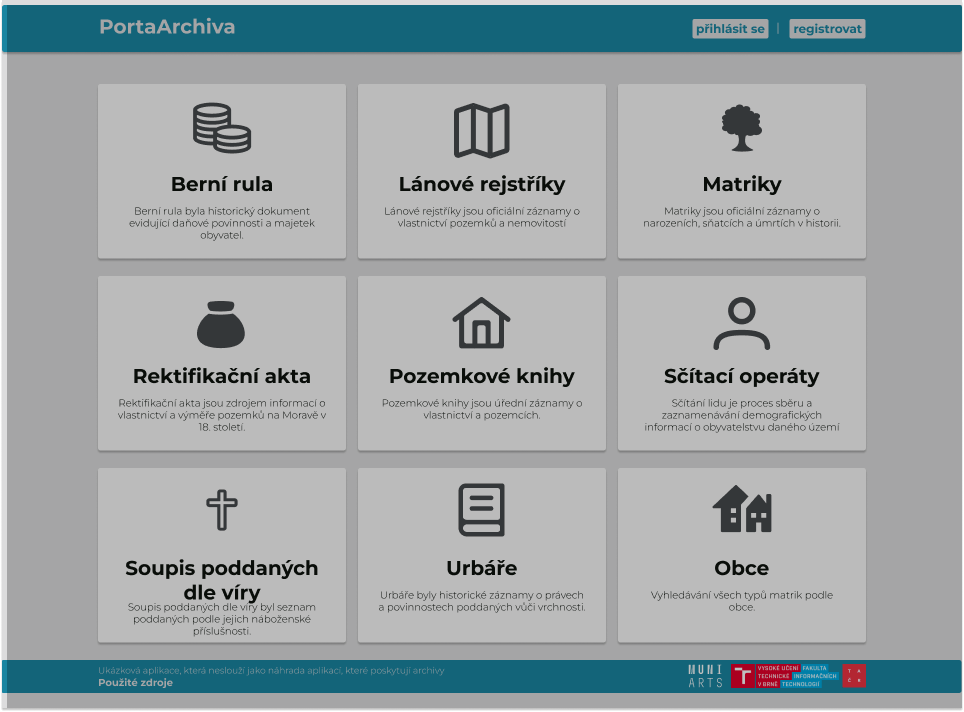
\includegraphics[scale=.35]{obrazky-figures/testing/figma-eye-defects/Main - Loss of Contrast.png}
    \caption{Hlavní strana - simulace Zeleného zákalu}
\end{figure}

\noindent
Deuteranopie je forma poruchy barvocitu, při níž pacient není schopen vnímat červenou barvu.
\begin{figure}[htbp]
\centering
    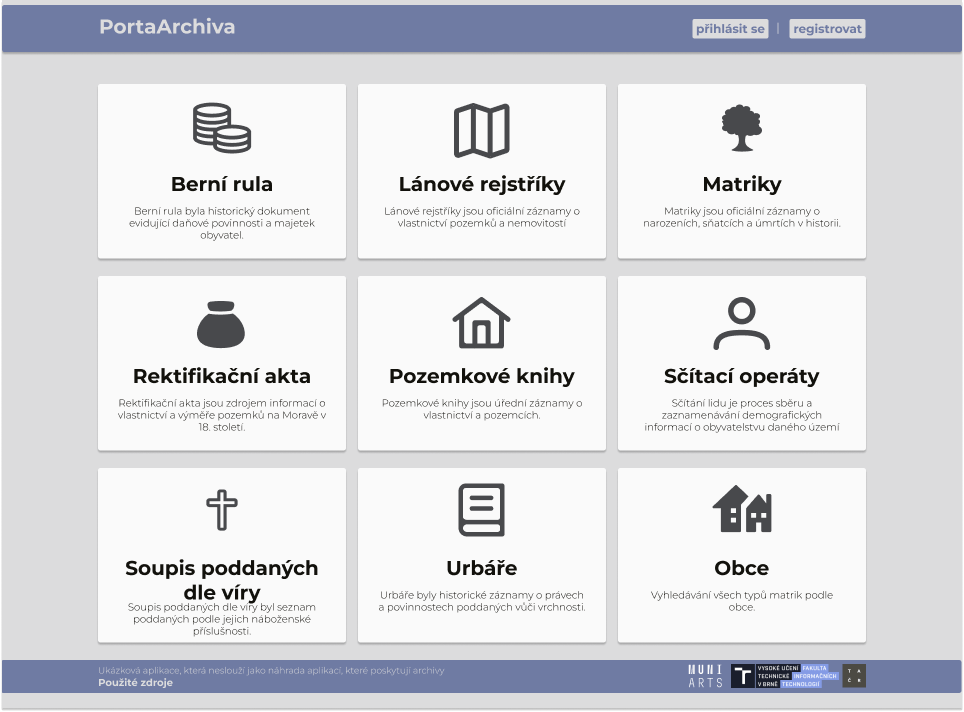
\includegraphics[scale=.35]{obrazky-figures/testing/figma-eye-defects/Main - Protanopia.png}
    \caption{Hlavní strana - simulace Protanopie}
\end{figure}

\newpage
\noindent
Deuteranopie je forma poruchy barvocitu, při níž pacient není schopen vnímat modrou barvu.
\begin{figure}[htbp]
\centering
    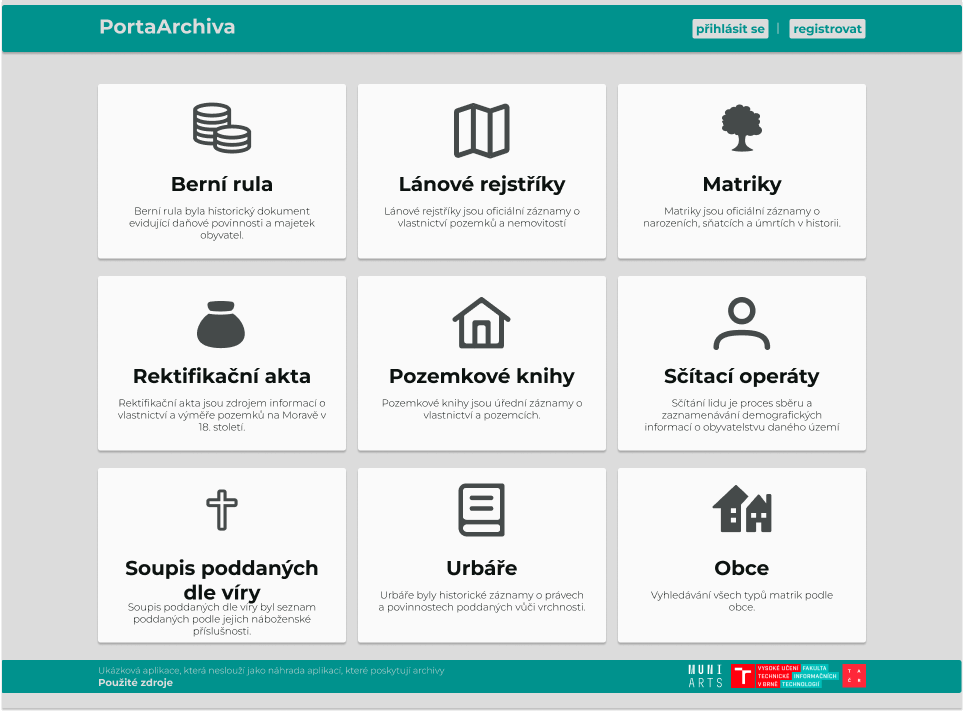
\includegraphics[scale=.35]{obrazky-figures/testing/figma-eye-defects/Main - Tritanopia.png}
    \caption{Hlavní strana - simulace Tritanopie}
\end{figure}

\noindent
Sedý zákal, nazývaný též katarakta, je onemocnění charakterizované zakalením čočky oka a způsobuje postupné zhoršování zrakové ostrosti.
\begin{figure}[htbp]
\centering
    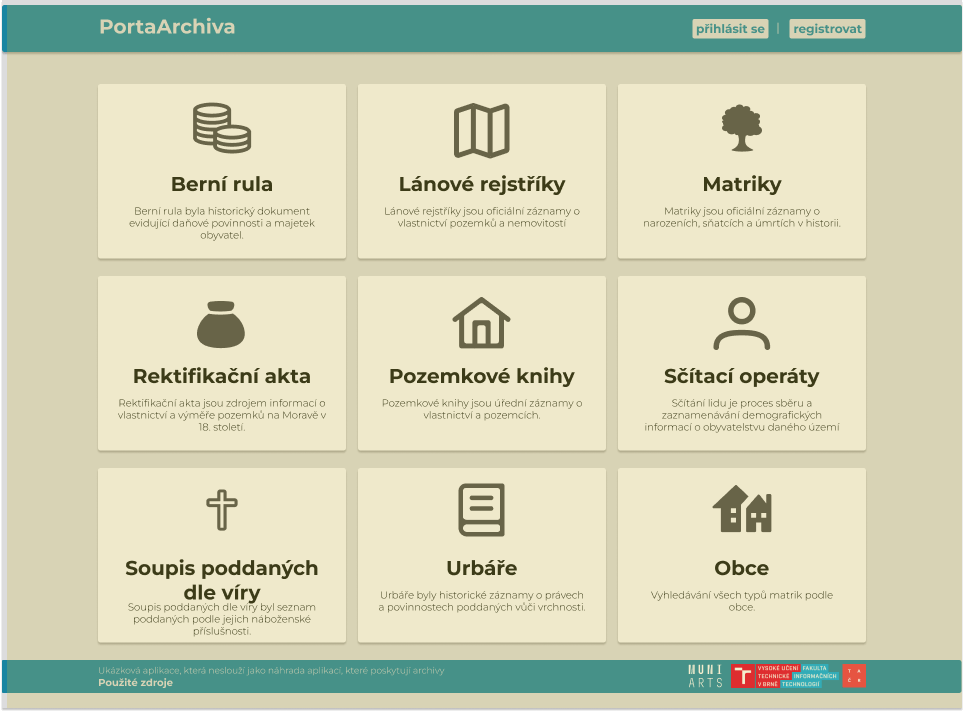
\includegraphics[scale=.35]{obrazky-figures/testing/figma-eye-defects/Main - Yellowing.png}
    \caption{Hlavní strana - simulace Šedého zákalu}
\end{figure}


\newpage
\section{Simulace očních vad pro prohlížeč archiválií}

Achromatopsie znamená úplnou barvoslepost, kdy oko nedokáže vnímat žádné barvy, což vede k tomu, že vidění je omezeno pouze na černou a bílou s odstíny šedi.
\begin{figure}[htbp]
\centering
    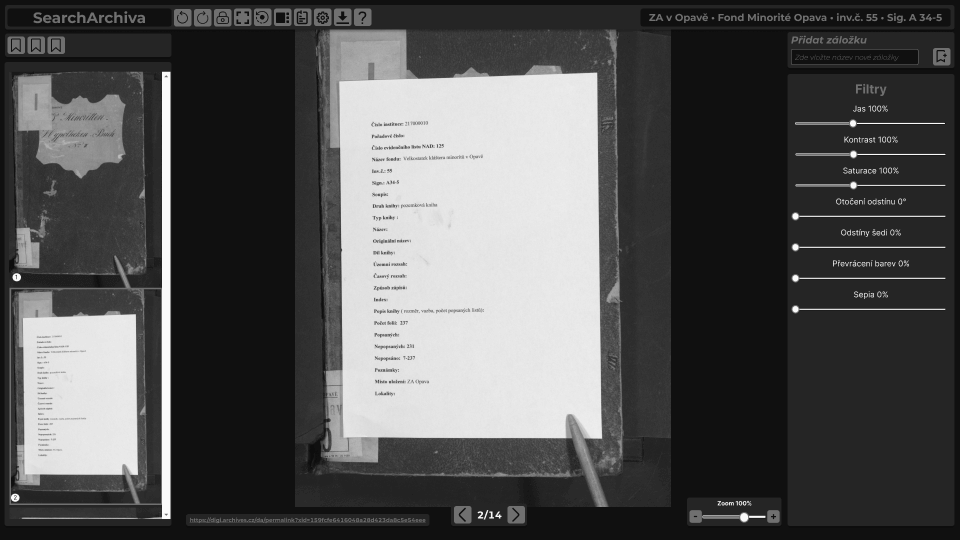
\includegraphics[scale=.35]{obrazky-figures/testing/figma-eye-defects/Gallery Page - Achromatopsia.png}
    \caption{Prohlížeč archiválií - simulace achromatopsie}
\end{figure}

\noindent
Oční vada, při které se paprsky světla, které procházejí čočkou lidského oka, sbíhají před sítnicí. Tím není na sítnici vytvořen ostrý obraz.
\begin{figure}[htbp]
\centering
    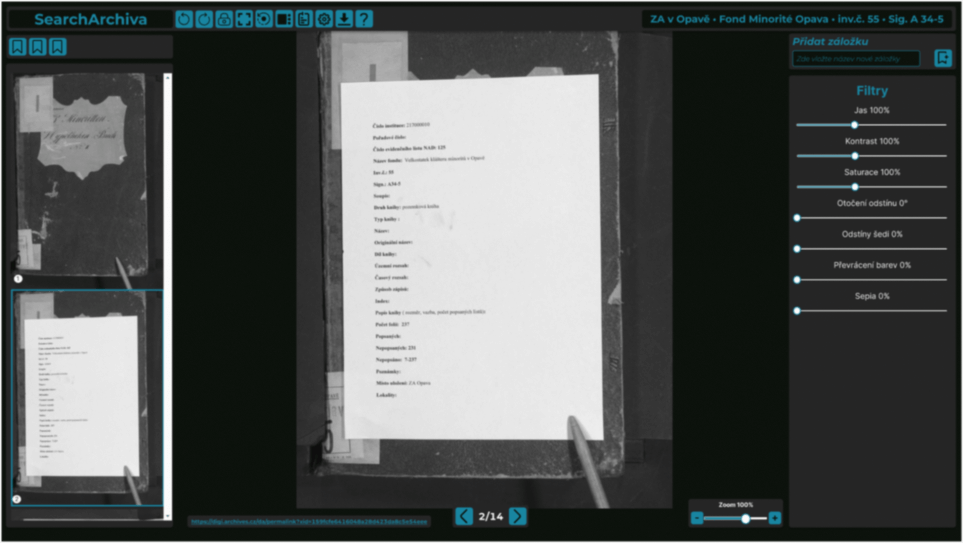
\includegraphics[scale=.35]{obrazky-figures/testing/figma-eye-defects/Gallery Page - Blurred.png}
    \caption{Prohlížeč archiválií - simulace krátkozrakosti}
\end{figure}

\newpage
\noindent
Světloplachost (fotofobie) se projevuje pocitem oslnění u pacientů i při pohledu za běžných světelných podmínek.
\begin{figure}[htbp]
\centering
    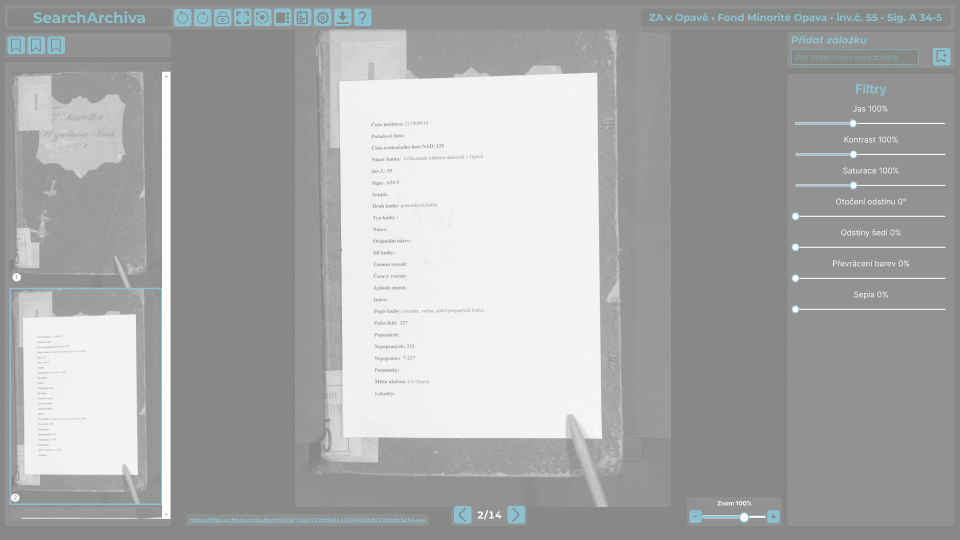
\includegraphics[scale=.35]{obrazky-figures/testing/figma-eye-defects/Gallery Page - Bright Light.png}
    \caption{Prohlížeč archiválií - simulace fotofobie}
\end{figure}

\noindent
Deuteranopie je forma poruchy barvocitu, při níž pacient není schopen vnímat zelenou barvu.
\begin{figure}[htbp]
\centering
    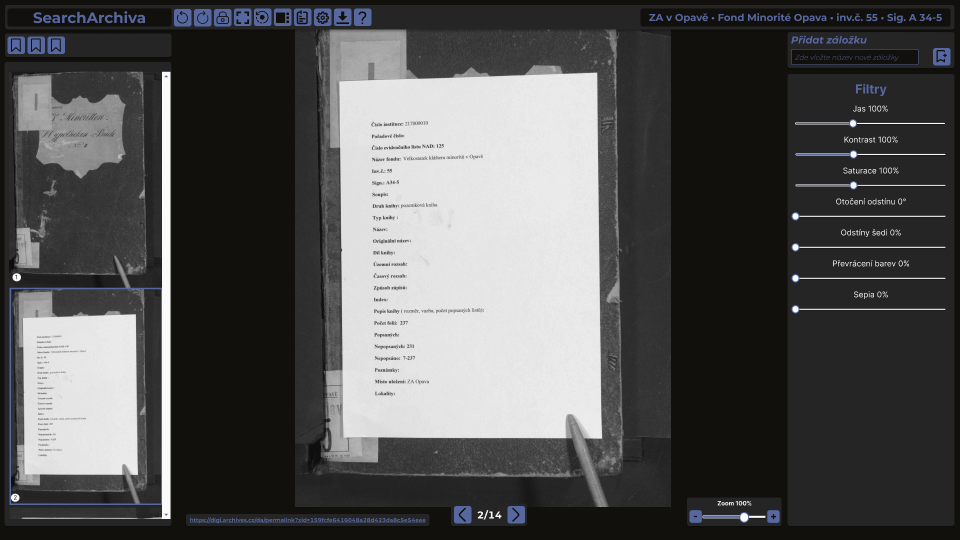
\includegraphics[scale=.35]{obrazky-figures/testing/figma-eye-defects/Gallery Page - Deuteranopia.png}
    \caption{Prohlížeč archiválií - simulace Deuteranopie}
\end{figure}

\newpage
\noindent
Diplopie je porucha, při níž pacient vnímá dva obrazy jednoho předmětu současně. Toto onemocnění se může také projevovat krátkodobým rozmazaným viděním.
\begin{figure}[htbp]
\centering
    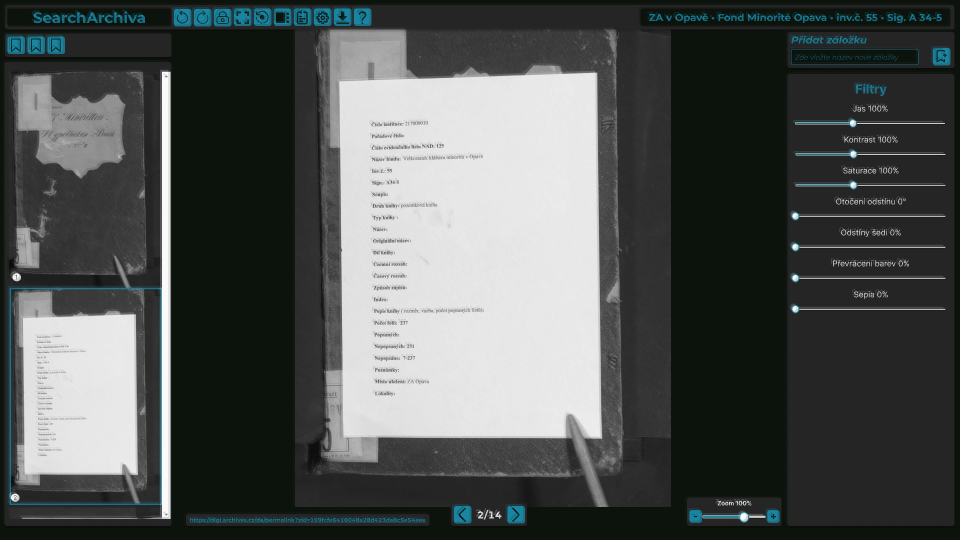
\includegraphics[scale=.35]{obrazky-figures/testing/figma-eye-defects/Gallery Page - Ghosting.png}
    \caption{Prohlížeč archiválií - simulace Diplopie}
\end{figure}

\noindent
Zelený zákal, lékařsky označovaný jako glaukom, je onemocnění, které způsobuje trvalé poškození zrakového nervu.
\begin{figure}[htbp]
\centering
    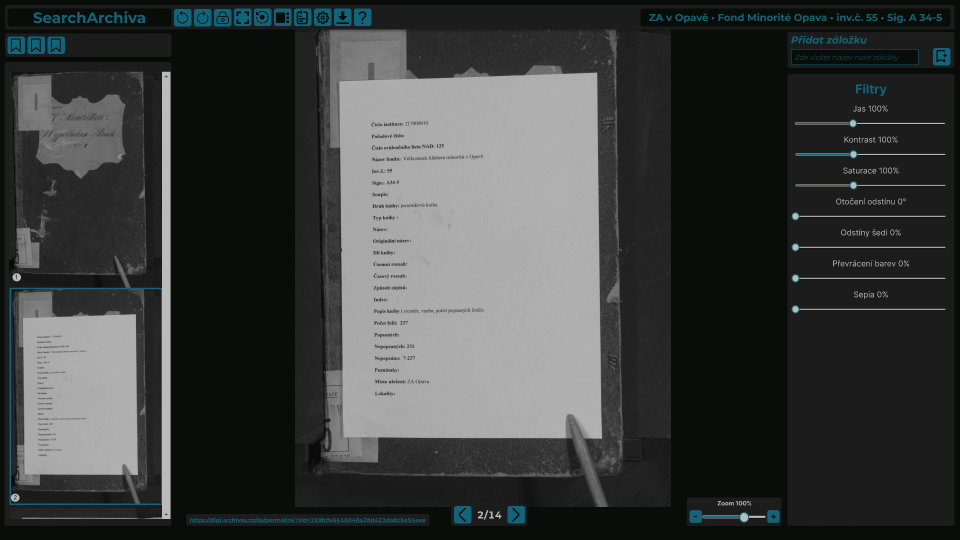
\includegraphics[scale=.35]{obrazky-figures/testing/figma-eye-defects/Gallery Page - Loss of Contrast.png}
    \caption{Prohlížeč archiválií - simulace Zeleného zákalu}
\end{figure}

\newpage
\noindent
Protanopie je forma poruchy barvocitu, při níž pacient není schopen vnímat červenou barvu.
\begin{figure}[htbp]
\centering
    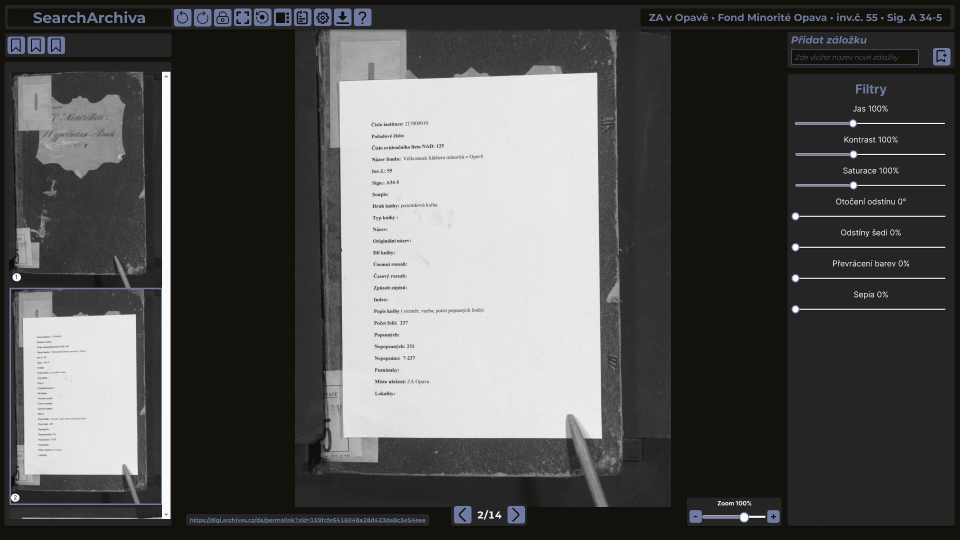
\includegraphics[scale=.35]{obrazky-figures/testing/figma-eye-defects/Gallery Page - Protanopia.png}
    \caption{Prohlížeč archiválií - simulace Protanopie}
\end{figure}

\noindent
Tritanopie je forma poruchy barvocitu, při níž pacient není schopen vnímat modrou barvu.
\begin{figure}[htbp]
\centering
    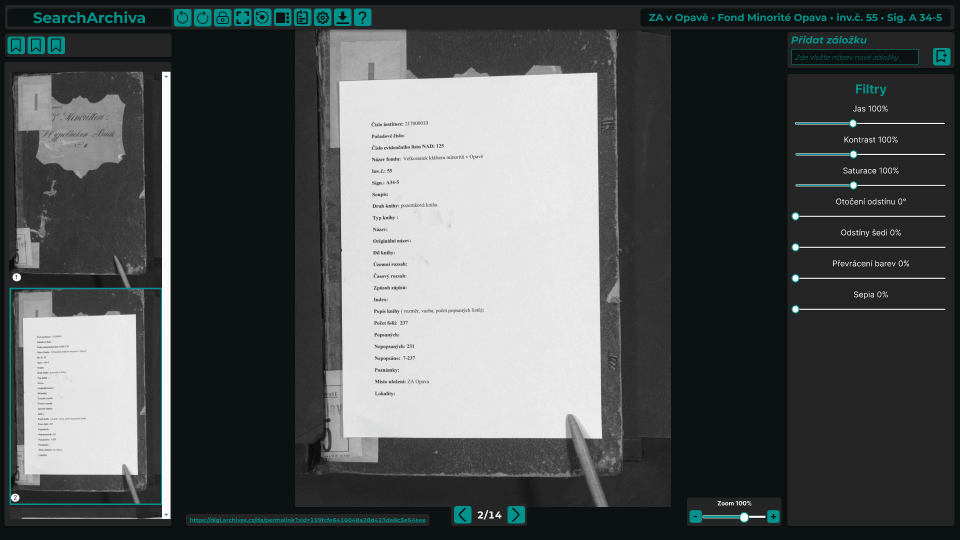
\includegraphics[scale=.35]{obrazky-figures/testing/figma-eye-defects/Gallery Page - Tritanopia.png}
    \caption{Prohlížeč archiválií - simulace Tritanopie}
\end{figure}

\newpage
\noindent
Šedý zákal, nazývaný též katarakta, je onemocnění charakterizované zakalením čočky oka a způsobuje postupné zhoršování zrakové ostrosti.
\begin{figure}[htbp]
\centering
    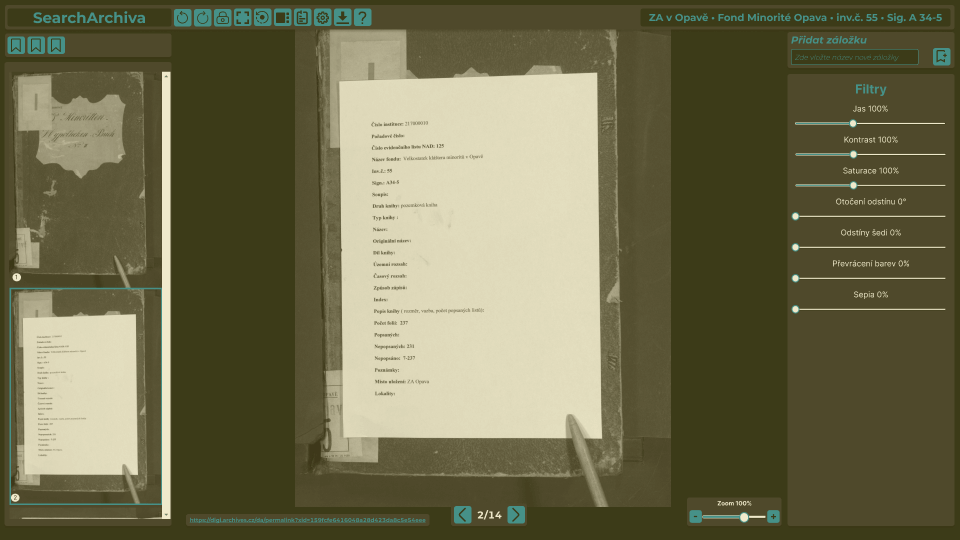
\includegraphics[scale=.35]{obrazky-figures/testing/figma-eye-defects/Gallery Page - Yellowing.png}
    \caption{Prohlížeč archiválií - simulace Šedého zákalu}
\end{figure}